
\providecommand{\Fun}{\operatorname{Fun}}
\providecommand{\Cat}{\mathcal{C}at}
\providecommand{\sSet}{s\mathcal{S}et}
\providecommand{\QCat}{\mathcal{Q}\mathcal{C}at}
\providecommand{\Disc}{\mathcal{D}\mathrm{isc}}  %
\providecommand{\qcOne}{\mathbf{1}}   %
\providecommand{\qcInt}{\mathbb{I}}   %
\providecommand{\rvWarrow}{\rightsquigarrow}%
\providecommand{\rvFarrow}{\twoheadrightarrow}%

\section{拟范畴富集的模型范畴}\label{sec:quasi-categorically-enriched-model-categories}

许多\trInfinityCosmos{}的例子，都以一个富集于 Joyal \trModelStructure{}之%
\trSimplicialSet{}上的\trModelCategory{}中\trCategoryOfFibrantObjects{}的形态出现%
——至少当一切\trFibrant{}对象皆\trCofibrant{}时如此，而出人意料的是，情形往往%
正是如此。\footnote{这一假设——一切\trFibrant{}对象皆\trCofibrant{}——对%
\trInfinityCategory{}理论的发展并非本质，尽管它确实使各种证明更为简省。事实上，
文献中首个「∞-宇宙」定义并未包含这一要求 \cite{bib110}。}例如，\trQuasiCategory{}的%
\trInfinityCosmos{}本身就以这种方式出现，因为 Joyal \trModelStructure{}是%
\trCartesianClosed{}（见第 1 章中的\cref{dig:joyal-model-structure}）。Joyal
\trModelStructure{}中的\trFibrant{}对象恰是诸\trQuasiCategory，\trFibrant{}对象之间的%
诸\trFibration{}恰是第 1 章中的\cref{def:isofibration}的诸\trIsofibration，而%
\trFibrant{}对象之间的诸\trWeakEquivalence{}恰是第 1 章中的%
\cref{def:equivalences-quasi-categories}的诸\trEquivalence。

\begin{proposition}\label{prop:fibrant-objects-cosmos}
试设 $\mathcal{M}$ 是任意一个富集于 Joyal \trModelStructure{}之上、且其中每个%
\trFibrant{}对象皆\trCofibrant{}的\trModelCategory。于是，\trFibrant{}对象的全子范畴
$\mathcal{M}_{f}$ 继承一个\trInfinityCosmos{}结构，其中诸\trIsofibration{}是%
\trFibrant{}对象之间的诸\trFibration，诸\trEquivalence{}是\trFibrant{}对象之间的诸%
\trWeakEquivalence，而诸\trTrivialFibration{}是\trFibrant{}对象之间的诸%
\trTrivialFibration。
\end{proposition}
\begin{proof}
由于 $\mathcal{M}$ 中的\trFibrant{}对象亦皆\trCofibrant，附录 C 中的%
\cref{lem:v-model-hom-fibrant}蕴含：$\mathcal{M}$ 中\trFibrant{}–\trCofibrant{}对象
之间的单纯富集 hom 都是\trQuasiCategory，我们将其记作 $\Fun(A,B)$。同一结果还蕴含：
对\trFibrant{}对象之间的任何\trFibration{} $f\colon A\rvFarrow B$，诱导映射
$f_{\ast}\colon\Fun(X,A)\rvFarrow\Fun(X,B)$ 是\trQuasiCategory{}的一个\trIsofibration。

由附录 C 中的\cref{exa:model-category-fibrant-objects}，诸\trFibrant{}对象连同其间
的诸\trFibration{}与诸\trWeakEquivalence{}定义了一个\trCategoryOfFibrantObjects
（见附录 C 中的\cref{def:category-of-fibrant-objects}）。特别地，非富集\trCategory
$\mathcal{M}_{f}$ 拥有一个\trTerminal{}对象、小\trProduct、诸\trIsofibration{}的%
\trPullback，以及诸\trIsofibration{}之可数塔的诸\trLimit，而这些\trLimit{}中的每一个
都在 $\mathcal{M}$ 中被创造。由于 $\mathcal{M}$ 容许单纯\trTensor，附录 A 中的%
\cref{prop:tensors-cotensors-conical}蕴含这些 1-范畴性的\trLimit{}都是锥形的，从而
$\mathcal{M}_{f}$ 拥有\cref{def:infinity-cosmos}(i) 的诸\trConicalLimit。诸%
\trIsofibration{}在\cref{def:infinity-cosmos}(ii) 的 1-范畴性\trLimit{}之下的稳定性，
随即也是附录 C 中的\cref{exa:model-category-fibrant-objects}之%
\trCategoryOfFibrantObjects{}结构的一部分，尽管在许多例子中，诸\trIsofibration{}类的
稳定性也可以经由附录 C 中的\cref{lem:right-lifting-closure}来建立。

尚须验证涉及单纯\trCotensor{}的诸公理。由假设，$\mathcal{M}$ 也余张量化于单纯集之上；
又因 $\mathcal{M}$ 是一个富集模型范畴，\trCotensor{}\trBifunctor{}是一个 Quillen 双变量%
\trAdjunction{}的\trRightAdjoint。直接从附录 C 中的%
\cref{def:quillen-two-variable-adjunction}的定义性公理可知：\trFibrant{}对象对与%
\trCofibrant{}对象作\trCotensor{}后封闭；但由于 Joyal \trModelStructure{}中的一切对象
皆\trCofibrant，\trFibrant{}对象对单纯\trCotensor{}封闭。于是 $\mathcal{M}_{f}$ 拥有
\cref{def:infinity-cosmos}(i) 的一切\trLimit。诸\trIsofibration{}的 Leibniz 稳定性则是
附录 C 中的\cref{def:quillen-two-variable-adjunction}的一个特例，这就证明了
$\mathcal{M}_{f}$ 是一个\trInfinityCosmos。

由于一切\trFibrant{}对象皆\trCofibrant，$\Fun(X,-)\colon\mathcal{M}_{f}\to\QCat$ 是
一支右 Quillen \trFunctor{}在\trFibrant{}对象上的作用（见附录 C 中的%
\cref{ex:quillen-bifunctor-component}），于是由附录 C 中的\cref{lem:quillen-preserves-we}，
$\mathcal{M}_{f}$ 中的诸\trWeakEquivalence{}被送到第 1 章中的%
\cref{def:equivalence-trivial-fibration}的诸\trEquivalence。反之，由第 1 章中的%
\cref{lem:equiv-homotopy-equivalences}，\trInfinityCosmos{}中的每个\trEquivalence{}都
容许一个\trHomotopyEquivalence{}结构——后者用 Quillen 会称之为「右同伦」
（right homotopies）的东西来定义。Quillen 证明：\trModelCategory{}中的任何%
\trHomotopyEquivalence{}都必定是一个\trWeakEquivalence{} \cite[\S1.1]{bib93}。
\end{proof}

再者：

\begin{corollary}\label{cor:right-quillen-adjunction-biequivalence}
任何介于诸拟范畴富集的模型范畴之间的、单纯富集的右 Quillen \trAdjunction——其中一切%
\trFibrant{}对象皆\trCofibrant{}——都定义一个\trCosmologicalFunctor，它每当该 Quillen
\trAdjunction{}定义一个 Quillen \trEquivalence{}时必是一个\trCosmologicalBiequivalence。
\end{corollary}
\begin{proof}
一支右 Quillen \trAdjunction{}保持\trFibrant{}对象，于是单纯富集的右 Quillen
\trAdjunction{}在诸\trFibrant{}对象的子范畴之间定义一个\trSimplicialFunctor，满足%
\trCosmologicalFunctor{}的第一条要求。作为一支右 Quillen \trFunctor，它保持%
\trFibrant{}对象之间的诸\trFibration，从而保持\cref{prop:fibrant-objects-cosmos}所
定义的诸\trInfinityCosmos{}中的诸\trIsofibration。最后，由附录 A 中的%
\cref{prop:enriched-adjoints-preserve-weighted-limits}，单纯富集的\trRightAdjoint{}%
同时保持锥形\trLimit{}与加权\trLimit。这就验证了定义\trCosmologicalFunctor{}的全部公理。

现在试考虑一个单纯富集的右 Quillen \trEquivalence{} $U\colon\mathcal{N}\to\mathcal{M}$，
连同其\trLeftAdjoint{} $F$。\trFunctor{} $U$ 在 hom 上的作用，同构于与一个余单位分量作
前复合所定义的映射：
\begin{center}
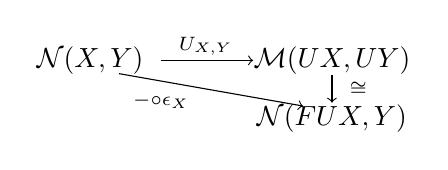
\begin{tikzpicture}[x=1.9em,y=1.5em]
  \node (tl) at (0,1.4) {$\mathcal{N}(X,Y)$};
  \node (tr) at (4.6,1.4) {$\mathcal{M}(UX,UY)$};
  \node (b)  at (4.6,0) {$\mathcal{N}(FUX,Y)$};
  \draw[->] (1.35,1.4) -- (3.1,1.4);
  \node at (2.2,1.74) {$\scriptstyle U_{X,Y}$};
  \draw[->] (0.55,1.08) -- (4.05,0.3);
  \node at (1.35,0.42) {$\scriptstyle -\circ\epsilon_X$};
  \draw[->] (4.6,1.05) -- (4.6,0.38);
  \node at (5.1,0.72) {$\scriptstyle\cong$};
\end{tikzpicture}
\end{center}
其中所示的竖直同构即伴随转置。由附录 C 中的\cref{lem:quillen-equivalence}，余单位分量
$\epsilon_X$ 在 $X$ 是\trFibrant{}的时是一个\trWeakEquivalence。当 $Y$ 是\trFibrant{}的
时，\trFunctor{} $\mathcal{N}(-,Y)\colon\mathcal{N}^{\mathrm{op}}\to\sSet$ 由附录 C 中
的\cref{ex:quillen-bifunctor-component}知是右 Quillen 的。于是，由附录 C 中的%
\cref{lem:quillen-preserves-we}，这一\trFunctor{}把 $\mathcal{N}$ 中\trCofibrant{}对象
之间的诸\trWeakEquivalence{}载为\trQuasiCategory{}之间的诸\trEquivalence。把这些合在一起
便知：当 $X$ 与 $Y$ 是\trFibrant{}的时，对角映射定义\trQuasiCategory{}的一个%
\trEquivalence，从而 $U_{X,Y}\colon\mathcal{N}(X,Y)\to\mathcal{M}(UX,UY)$ 也必定是%
\trQuasiCategory{}的一个\trEquivalence。这就验证了\trCosmologicalBiequivalence{}的%
\trLocalEquivalence{}性质。

本质满性也是附录 C 中的\cref{lem:quillen-equivalence}的一个推论，因为导出单位对任何%
\trFibrant{}对象 $M\in\mathcal{M}$ 都给出一个\trWeakEquivalence{} $M\rvWarrow URFM$。
由于 $RFM$ 是 $\mathcal{N}$ 中的一个\trFibrant{}对象，这就在\trInfinityCosmos{}
$\mathcal{M}_{f}$ 中定义了一个\trEquivalence，涉及 $U\colon\mathcal{N}_{f}\to\mathcal{M}_{f}$
像中的一个对象。
\end{proof}

有了\cref{prop:fibrant-objects-cosmos}，下一个问题便是：富集于 Joyal \trModelStructure{}%
之上的诸\trModelCategory{}从何而来？这一问题在文献中未受多少关注，但在许多情形，相关学界
帮了我们一个大忙：他们提供了由无穷维\trCategory{}组成、却富集于其他某个\trCartesianClosed
\trModelCategory{}之上的诸\trModelCategory。这使我们得以施用附录 C 中的%
\cref{thm:change-of-base-quillen-model}，把一个已知的富集转换为对 Joyal 拟范畴%
\trModelStructure{}的富集。把该结果与\cref{prop:fibrant-objects-cosmos}结合起来，我们便
得到一个有用的\trChangeOfBase{}结果，它产出富集于 Joyal \trModelStructure{}之上的诸%
\trModelCategory。

\begin{proposition}\label{prop:change-of-base-model-cosmoi}
试设 $\mathcal{V}$ 是一个\trCartesianClosed{}模型范畴，它配备一个 Quillen
\trAdjunction，其\trRightAdjoint{}取值于 Joyal \trModelStructure{}，而其\trLeftAdjoint{}%
保持有限\trProduct{}：
\begin{center}
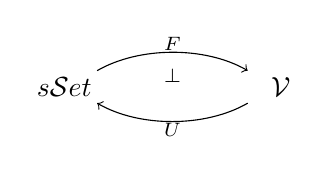
\begin{tikzpicture}[x=1.7em,y=1.4em]
  \node (s) at (0,0) {$\sSet$};
  \node (v) at (4.6,0) {$\mathcal{V}$};
  \draw[->] (0.7,0.42) .. controls (1.6,1.05) and (3.0,1.05) .. (3.9,0.42);
  \node at (2.3,1.12) {$\scriptstyle F$};
  \node at (2.3,0.28) {$\scriptstyle\bot$};
  \draw[->] (3.9,-0.42) .. controls (3.0,-1.05) and (1.6,-1.05) .. (0.7,-0.42);
  \node at (2.3,-1.12) {$\scriptstyle U$};
\end{tikzpicture}
\end{center}
\begin{enumerate}[label=(\roman*)]
\item 则对任何其中每个\trFibrant{}对象皆\trCofibrant{}的 $\mathcal{V}$-模型范畴
  $\mathcal{M}$，\trFibrant{}对象的全子范畴 $\mathcal{M}_{f}$ 定义一个\trInfinityCosmos，
  其中诸\trIsofibration{}是\trFibrant{}对象之间的诸\trFibration，诸\trEquivalence{}是%
  \trFibrant{}对象之间的诸\trWeakEquivalence，诸\trTrivialFibration{}是\trFibrant{}对象
  之间的诸\trTrivialFibration；诸\trFunctorSpace{}由
  $\Fun(M,N)\coloneqq U\mathcal{M}(M,N)$ 定义——其中 $\mathcal{M}(M,N)$ 是 $\mathcal{V}$
  中的 hom-对象；而 $M\in\mathcal{M}_{f}$ 与 $S\in\sSet$ 的单纯\trCotensor{}则由
  $\mathcal{V}$-\trCotensor{} $M^{FS}$ 定义。
\item 此外，任何介于诸此形 $\mathcal{V}$-模型范畴之间的右 Quillen $\mathcal{V}$-伴随都
  定义一个\trCosmologicalFunctor，它每当该 Quillen \trAdjunction{}是一个 Quillen
  \trEquivalence{}时必是一个\trCosmologicalBiequivalence。
\end{enumerate}
\end{proposition}
\begin{proof}
伴随 $F\dashv U$ 被假设为介于诸\trCartesianClosed{}模型范畴之间的一个 Quillen
\trAdjunction，其中\trLeftAdjoint{}保持有限\trProduct。于是，由附录 C 中的%
\cref{thm:change-of-base-quillen-model}，任何 $\mathcal{V}$-模型范畴 $\mathcal{M}$ 都
容有成为一个富集于 Joyal \trModelStructure{}之上的\trModelCategory{}的结构，后者具有
同一个底层非富集模型范畴，其富集 hom 与\trCotensor{}定义为：
\[
\Fun(M,N)\coloneqq U\mathcal{M}(M,N)
\qquad\text{以及}\qquad
M^{S}\coloneqq M^{FS},
\]
如所断言。由于底层模型范畴未曾改变，$\mathcal{M}$ 中的每个\trFibrant{}对象仍是%
\trCofibrant{}的。于是，由\cref{prop:fibrant-objects-cosmos}，\trFibrant{}对象的全子范畴
定义一个\trInfinityCosmos。

再者，由于这一\trChangeOfBase{}结果不影响诸底层模型范畴，任何介于诸 $\mathcal{V}$-模型
范畴之间的右 Quillen 伴随都仍是一支右 Quillen 伴随。由附录 A 中的%
\cref{prop:change-of-base-2-functor}，一个 $\mathcal{V}$-\trFunctor{}在新富集之下成为
单纯富集的\trFunctor。\cref{cor:right-quillen-adjunction-biequivalence}现在告诉我们：
一支右 Quillen $\mathcal{V}$-伴随产生一个\trCosmologicalFunctor，它在那个 Quillen 伴随
是一个 Quillen \trEquivalence{}时是一个\trCosmologicalBiequivalence。
\end{proof}

我们常常在如下特殊情形中利用这一结果：

\begin{corollary}\label{cor:cartesian-closed-cosmos}
试设 $\mathcal{V}$ 是一个其中每个\trFibrant{}对象皆\trCofibrant{}的\trCartesianClosed{}%
模型范畴，它配备一个 Quillen \trAdjunction，其\trRightAdjoint{}取值于 Joyal
\trModelStructure{}，而其\trLeftAdjoint{}保持有限\trProduct{}：
\begin{center}
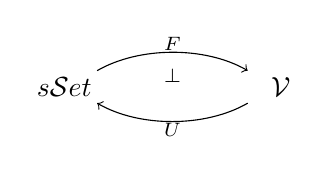
\begin{tikzpicture}[x=1.7em,y=1.4em]
  \node (s) at (0,0) {$\sSet$};
  \node (v) at (4.6,0) {$\mathcal{V}$};
  \draw[->] (0.7,0.42) .. controls (1.6,1.05) and (3.0,1.05) .. (3.9,0.42);
  \node at (2.3,1.12) {$\scriptstyle F$};
  \node at (2.3,0.28) {$\scriptstyle\bot$};
  \draw[->] (3.9,-0.42) .. controls (3.0,-1.05) and (1.6,-1.05) .. (0.7,-0.42);
  \node at (2.3,-1.12) {$\scriptstyle U$};
\end{tikzpicture}
\end{center}
则 $\mathcal{V}$ 的诸\trFibrant{}对象定义一个\trCartesianClosed{}\trInfinityCosmos{}
$\mathcal{V}_{f}$，且其\trRightAdjoint{}定义一个\trCosmologicalFunctor{}
$U\colon\mathcal{V}_{f}\to\QCat$，后者自然同构于底\trQuasiCategory\trFunctor，并每当
$F\dashv U$ 是一个 Quillen \trEquivalence{}时必是一个\trCosmologicalBiequivalence。
\end{corollary}
\begin{proof}
当 $\mathcal{V}$ 的\trFibrant{}对象皆\trCofibrant{}时，$\mathcal{V}$ 本身满足%
\cref{prop:change-of-base-model-cosmoi}(i) 的假设，从而 $\mathcal{V}_{f}$ 定义一个%
\trInfinityCosmos。由附录 A 中的\cref{lem:finite-product-adjunction-v-enriched}，
$F\dashv U$ 在单纯集与单纯富集\trCategory{} $U_{*}\mathcal{V}$ 之间定义一个单纯富集的%
\trAdjunction，这样我们便得到一支单纯富集的右 Quillen \trFunctor{}
$U\colon U_{*}\mathcal{V}\to\sSet$，介于富集于 Joyal \trModelStructure{}之上的诸模型范畴
之间。由\cref{cor:right-quillen-adjunction-biequivalence}，$U$ 进而定义一个%
\trCosmologicalFunctor{} $U\colon\mathcal{V}_{f}\to\QCat$，它在 $F\dashv U$ 是一个
Quillen \trEquivalence{}时是一个\trBiequivalence。把附录 A 中的%
\cref{rem:exponent-one-identity}与\cref{prop:change-of-base-model-cosmoi}所给出的
$\mathcal{V}_{f}$ 之诸\trFunctorSpace{}的定义结合起来，对任何 $X\in\mathcal{V}_{f}$ 我们
便得到下述自然\trIsomorphism
\[
U(X)\cong U(X^{1})\cong\Fun(1,X)
\]
这就证明了\trCosmologicalFunctor{} $U\colon\mathcal{V}_{f}\to\QCat$ 自然同构于配属于%
\trInfinityCosmos{} $\mathcal{V}_{f}$ 的底\trQuasiCategory\trFunctor（另见第 1 章中的%
\cref{rem:underlying-qcat-internal-homs}）。
\end{proof}

\cref{prop:change-of-base-model-cosmoi}启发了如下\trInfinityCosmos{}的平凡例子。

\begin{example}[作为∞-宇宙的 1-范畴]\label{exa:one-categories-as-cosmoi}
任何\trComplete{}且\trLocallySmall $1$-\trCategory{} $\mathcal{E}$ 都可以被造就成一个%
\trInfinityCosmos，其中 $\Fun(A,B)$ 恰是从 $A$ 到 $B$ 的态射之集。由\trYonedaLemma，此时的
诸\trEquivalence{}便是 $\mathcal{E}$ 中的诸\trIsomorphism，于是由第 1 章中的%
\cref{lem:brown-factorization}，一切映射都必定是\trIsofibration。$\mathcal{E}$ 中对象
$A$ 与一个\trSimplicialSet{} $S$ 的\trCotensor{}定义为
\[
A^{S}\coloneqq A^{\pi_{0}S}\coloneqq\prod_{\pi_{0}S}A.
\]
\end{example}

姑且不顾\trModelCategory{}通常被假定除\trLimit{}外还拥有\trColimit{}这一事实，此构造可以
看作\cref{prop:change-of-base-model-cosmoi}施于伴随
\begin{center}
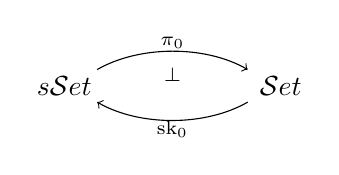
\begin{tikzpicture}[x=1.7em,y=1.4em]
  \node (s) at (0,0) {$\sSet$};
  \node (v) at (4.6,0) {$\mathcal{S}et$};
  \draw[->] (0.7,0.42) .. controls (1.6,1.05) and (3.0,1.05) .. (3.9,0.42);
  \node at (2.3,1.12) {$\scriptstyle\pi_{0}$};
  \node at (2.3,0.28) {$\scriptstyle\bot$};
  \draw[->] (3.9,-0.42) .. controls (3.0,-1.05) and (1.6,-1.05) .. (0.7,-0.42);
  \node at (2.3,-1.12) {$\scriptstyle\mathrm{sk}_{0}$};
\end{tikzpicture}
\end{center}
的一个特例，其\trRightAdjoint{}把 $\mathcal{S}et$ 作为由 0-骨架单纯集构成的子范畴嵌入
$\sSet$（见附录 C 中的\cref{def:simplex-skeleton-coskeleton}）。此处 $\mathcal{S}et$ 上的%
\trCartesianClosed\trModelStructure{}并非附录 C 中的\cref{ex:set-model-category}所考虑的
那一个，而是其中诸\trWeakEquivalence{}为诸\trIsomorphism、一切映射都同时取作余纤维化与
纤维化的那一个。为见这一伴随是 Quillen 的，注意 $\pi_{0}$ 空洞地保持余纤维化，而
$\mathrm{sk}_{0}$ 把任何映射载为\trQuasiCategory{}的一个\trIsofibration：后一断言经由
伴随可得，因为下方左侧的定义性提升性质经转置便给出下方右侧的提升性质：
\begin{center}
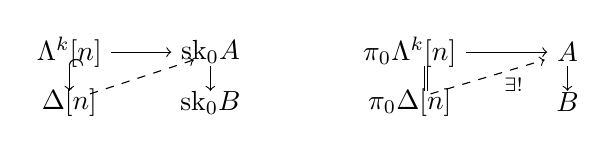
\begin{tikzpicture}[x=1.5em,y=1.4em]
  \node (tl) at (0,1.3) {$\Lambda^k[n]$};
  \node (tr) at (3.4,1.3) {$\mathrm{sk}_{0}A$};
  \node (bl) at (0,0) {$\Delta[n]$};
  \node (br) at (3.4,0) {$\mathrm{sk}_{0}B$};
  \draw[->] (tl) -- (tr);
  \draw[->] (0,0.95) -- (0,0.3);
  \draw (0,0.95) arc[start angle=180,end angle=0,radius=0.16];
  \draw[->,dashed] (0.5,0.22) -- (3.0,1.1);
  \draw[->] (3.4,0.95) -- (3.4,0.3);
  \node at (6.0,0.65) {$\leftrightsquigarrow$};
  \begin{scope}[shift={(8.2,0)}]
    \node (tl2) at (0,1.3) {$\pi_{0}\Lambda^k[n]$};
    \node (tr2) at (3.8,1.3) {$A$};
    \node (bl2) at (0,0) {$\pi_{0}\Delta[n]$};
    \node (br2) at (3.8,0) {$B$};
    \draw[->] (tl2) -- (tr2);
    \draw[double] (0.4,0.95) -- (0.4,0.3);
    \draw[->,dashed] (0.5,0.22) -- (3.25,1.1);
    \node at (2.5,0.45) {$\scriptstyle\exists!$};
    \draw[->] (3.8,0.95) -- (3.8,0.3);
  \end{scope}
\end{tikzpicture}\\[1.2ex]
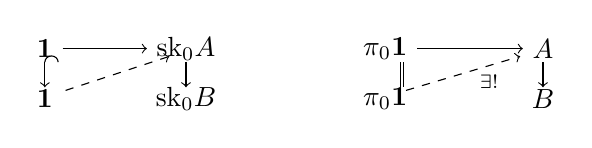
\begin{tikzpicture}[x=1.5em,y=1.4em]
  \node (tl) at (0,1.3) {$\qcOne$};
  \node (tr) at (3.4,1.3) {$\mathrm{sk}_{0}A$};
  \node (bl) at (0,0) {$\qcOne$};
  \node (br) at (3.4,0) {$\mathrm{sk}_{0}B$};
  \draw[->] (tl) -- (tr);
  \draw[->] (0,0.95) -- (0,0.3);
  \draw (0,0.95) arc[start angle=180,end angle=0,radius=0.16];
  \draw[->,dashed] (0.5,0.22) -- (3.0,1.1);
  \draw[->] (3.4,0.95) -- (3.4,0.3);
  \node at (6.0,0.65) {$\leftrightsquigarrow$};
  \begin{scope}[shift={(8.2,0)}]
    \node (tl2) at (0,1.3) {$\pi_{0}\qcOne$};
    \node (tr2) at (3.8,1.3) {$A$};
    \node (bl2) at (0,0) {$\pi_{0}\qcOne$};
    \node (br2) at (3.8,0) {$B$};
    \draw[->] (tl2) -- (tr2);
    \draw[double] (0.4,0.95) -- (0.4,0.3);
    \draw[->,dashed] (0.5,0.22) -- (3.25,1.1);
    \node at (2.5,0.45) {$\scriptstyle\exists!$};
    \draw[->] (3.8,0.95) -- (3.8,0.3);
  \end{scope}
\end{tikzpicture}
\end{center}
众所周知，$\pi_{0}$ 保持有限\trProduct{}，于是\trChangeOfBase{}定理的条件成立。以此方式
产生的\trInfinityCosmos{}之\trHomotopyTwoCategory{}只有恒同 2-\trCell。

\begin{example}[作为∞-宇宙的 2-范畴]\label{exa:two-categories-as-cosmoi}
将上一例范畴化，任何带充分极限的 $2$-\trCategory{} $\mathcal{E}$ 都定义一个%
\trInfinityCosmos，其中 $\Fun(A,B)$ 是 $\mathcal{E}$ 中从 $A$ 到 $B$ 的态射之
hom-\trCategory{}的\trNerve。由第 1 章中的\cref{thm:equivalences-are-equivalences}与
附录 B 中的\cref{prop:equivalences-representably-defined}，诸\trEquivalence{}必定是该
$2$-\trCategory{}中的诸\trEquivalence。受第 1 章中的%
\cref{prop:isofibrations-are-isofibrations}启发，我们取诸\trIsofibration{}为该
$2$-\trCategory{}中的诸\trIsofibration。
\end{example}

若把「充分极限」解作\cref{def:infinity-cosmos}(i) 的诸\trLimit，则剩下的公理%
\cref{def:infinity-cosmos}(ii) 可以手工验证。或者，再一次不顾\trModelCategory{}通常被
假定除\trLimit{}外还拥有\trColimit{}这一事实，我们可以把%
\cref{prop:change-of-base-model-cosmoi}施于第 1 章中的\cref{prop:nerve-left-adjoint}的
同伦范畴$\dashv$\trNerve{}\trAdjunction
\begin{center}
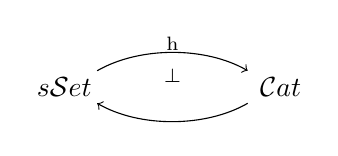
\begin{tikzpicture}[x=1.7em,y=1.4em]
  \node (s) at (0,0) {$\sSet$};
  \node (v) at (4.6,0) {$\Cat$};
  \draw[->] (0.7,0.42) .. controls (1.6,1.05) and (3.0,1.05) .. (3.9,0.42);
  \node at (2.3,1.12) {$\scriptstyle\mathrm{h}$};
  \node at (2.3,0.28) {$\scriptstyle\bot$};
  \draw[->] (3.9,-0.42) .. controls (3.0,-1.05) and (1.6,-1.05) .. (0.7,-0.42);
\end{tikzpicture}
\end{center}
——它是 Joyal \trModelStructure{}与范畴上常见的「民俗」模型结构之间的一个 Quillen
\trAdjunction。任何容有适当有限\trLimit{}与\trColimit{}的 $2$-\trCategory，在配备由
Lack \cite{bib72} 所描述的「平凡」$\Cat$-富集模型结构时，便典范地富集于范畴的民俗模型
结构之上，其弱等价与纤维化恰是刚才描述的那些\trEquivalence{}与\trIsofibration。

尚须揭开「充分极限」这一含糊措辞的含义。由第 6 章中的%
\cref{prop:flexible-weights-homotopical}，$2$-\trCategory{} $\mathcal{E}$ 被要求拥有一切
PIE 极限，即第 6 章中的\cref{dig:flexible-2-limits}所讨论的 2-范畴性的\trProduct、插入子
与均衡化子。据第 6 章中的\cref{def:iso-commas}的构造，这蕴含 $\mathcal{E}$ 容有全部映射
的拟拉回（pseudopullback），但这并不完全蕴含 $\mathcal{E}$ 容有诸\trIsofibration{}的
2-拉回。确切地说，第 6 章中的\cref{lem:iso-commas-pullbacks}之证明构造了一个%
\trIsofibration{}的双拉回（bipullback），其中通常的 hom-\trCategory{}同构被替换为一个
hom-\trCategory{}等价。类似的议论适用于诸\trIsofibration{}之塔的诸\trLimit。但在实践中，
容有 PIE 极限的诸 $2$-\trCategory——例如 \cite{bib18} 所考虑的那些——看来确实容有诸%
\trIsofibration{}的 2-拉回与诸\trIsofibration{}之塔的 2-极限，从而定义出\trInfinityCosmos
的例子。

特别地，把\cref{exa:two-categories-as-cosmoi}特化，便复原出第 1 章中的%
\cref{prop:cosmos-categories}所讨论的 $\Cat$ 上的\trInfinityCosmos{}结构。有趣的是，它也
在 $\Cat^{\mathrm{op}}$ 上定义一个\trInfinityCosmos{}结构，其中的「\trIsofibration」是
那些在对象上单射的\trFunctor。\footnote{在 $\Cat$ 的「民俗」模型结构中，诸纤维化是诸%
\trIsofibration，诸弱等价是诸\trEquivalence，而诸余纤维化是在对象上单射的诸\trFunctor。
在对象上单射的函子满足一个同构扩张性质，它与定义 2-范畴性\trIsofibration{}概念的那个同构
提升性质相对偶。}把这些观察与第 1 章中的\cref{def:co-dual-cosmoi}的对偶∞-宇宙构造结合
起来，便可见四个 2-范畴性的对偶 $\Cat$、$\Cat^{\mathrm{op}}$、$\Cat^{\mathrm{co}}$ 与
$\Cat^{\mathrm{coop}}$ 全都是\trInfinityCosmos。

\cref{exa:two-categories-as-cosmoi}的诸\trInfinityCosmos{}容有一个抽象刻画：它们恰是那些
（作为拟范畴富集的范畴）同构于自身\trHomotopyTwoCategory{}的\trInfinityCosmos。在此情形，
第 3 章中的诸弱 2-极限实际上是严格的，而我们的许多结果都可特化为 2-范畴论文献中已知的定理。

\begin{example}[作为∞-宇宙的单纯模型范畴]\label{exa:simplicial-model-categories-as-cosmoi}
恒同\trFunctor{} $\mathrm{id}\colon\sSet\to\sSet$ 定义一支从 Quillen 的 Kan 复形模型结构
到 Joyal 的拟范畴模型结构的右 Quillen 伴随；显然，其\trLeftAdjoint{}保持\trProduct。于是，
任何 Kan 复形富集的模型范畴——或按惯常的说法，\textbf{单纯模型范畴}
（simplicial model category）——都可以视为一个拟范畴富集的模型范畴，其中\trFibrant{}–%
\trCofibrant{}对象之间的每个\trMappingSpace{}都恰好是一个 Kan 复形。从而，任何\trFibrant{}%
对象皆\trCofibrant{}的单纯模型范畴都可以视为呈现了一个\trInfinityCosmos。
\end{example}

以此方式产生的诸\trHomotopyTwoCategory{}都是 $(2,1)$-\trCategory，其中每个%
\trNaturalTransformation{}都定义一个自然\trIsomorphism。

\begin{digression}[论可达∞-宇宙]\label{dig:accessible-cosmoi}
人们在实践中遇到的许多模型范畴——包括本书考虑的一切例子——都是\emph{组合的}
（combinatorial），意即底范畴是局部可表现的（locally presentable），而模型结构是余纤维性
生成的（cofibrantly generated）。当满足\cref{prop:fibrant-objects-cosmos}之假设的一个
模型范畴 $\mathcal{M}$ 是组合的时，所得的\trInfinityCosmos{} $\mathcal{M}$ 便是一个%
\textbf{可达\trInfinityCosmos}（accessible $\infty$-cosmos）——这是 Bourke 与 Lack 正在研究的
一个概念，它基于他们早先与 Vokřínek 就同伦伴随函子定理所做的合作工作 \cite{bib22}。事实上，
第 6 章中的诸构造很可能都保持可达性，果真如此，则本书考虑的每一座\trInfinityCosmos{}都是
可达的。
\end{digression}

这一观察将有不可胜数的应用留待未来的工作去探究，它们源于把 \cite{bib22} 的主定理特化到这一
情境。首先，任何可达\trInfinityCosmos{}都拥有一切\textbf{柔性加权同伦余极限}，其定义由形如附录 A 中
的\cref{def:weighted-limit-colimit-universal-property}的一个单纯富集泛性质给出，只是以%
\trQuasiCategory{}的\trEquivalence{}而非\trIsomorphism{}来表述。\footnote{\eqref{eq:weighted-universal-property}
中的一切单纯集都是\trQuasiCategory，这一事实是权之柔性的一项推论（见第 6 章中的%
\cref{def:flexible-weights}与\cref{prop:flexible-weights-homotopical}）。}这一结果本身
可以理解为一则第二定理的推论，后者断言：任何介于诸可达\trInfinityCosmos{}之间、作为非富集%
\trFunctor{}为可达的\trCosmologicalFunctor{} $U\colon\mathcal{K}\to\mathcal{L}$ 都容有一个
同伦性的左伴随：对每个 $A\in\mathcal{L}$，都存在 $FA\in\mathcal{K}$ 连同一个映射
$\eta_{A}\colon A\to UFA$，后者对一切 $B\in\mathcal{K}$ 诱导\trQuasiCategory{}的一个%
\trEquivalence
\[
\Fun(FA,B)\rvWarrow \Fun(A,UB)
\]
例如，宇宙论嵌入 $\Disc(\mathcal{K})\hookrightarrow\mathcal{K}$ 恰当 $\mathcal{K}$ 是一个
可达\trInfinityCosmos{}时是可达的，于是这一结果定义了一个弱反射（weak reflection）——它
「自由地逆转」某座\trInfinityCategory{}中的全部箭头。

\subsection*{练习}

\begin{exercise}\label{ex:enriched-fibrant-object-categories}
陈述并证明\cref{prop:change-of-base-model-cosmoi}的一个版本，使之适用于富集的%
\trCategoryOfFibrantObjects——例如\cref{exa:one-categories-as-cosmoi}与%
\cref{exa:two-categories-as-cosmoi}中所考虑的那些——此类范畴可以几乎没有余极限。
\end{exercise}

